\section{The State-of-Art Approach}
\label{sec:soa}
Before presenting our solution {\methodName}, we first describe the state-of-art graph anonymization approach ({\soaName})~\cite{Boldi_Injecting_2012} in the deterministic scenario. 
The purpose of describing it is to separate the basic framework with the contribution of {\methodName}. 
They differ in the search strategy of sanitized candidates.  

\subsection{Overview}~~
The {\soaName} method obfuscates the (deterministic) graph data by adding or removing edges \emph{partially}. 
For each edge $e$, it assigns a probabilistic deviation $r_{e} \in [0,1]$, where $r_{e} \leftarrow R(\sigma)$. 
In particular, the uncertainty injecting scheme proceeds as follows:
\begin{equation}
    p(e) =
    \begin{cases}
         1-r_{e}  & e \in E \\
         r_{e}    & otherwise 
    \end{cases}
    \label{eq:inject}
\end{equation}
Generally, it transfers edge existence from existing edges to non-existing ones for identification obfuscation.   

\begin{figure}[htb]
  \centering
        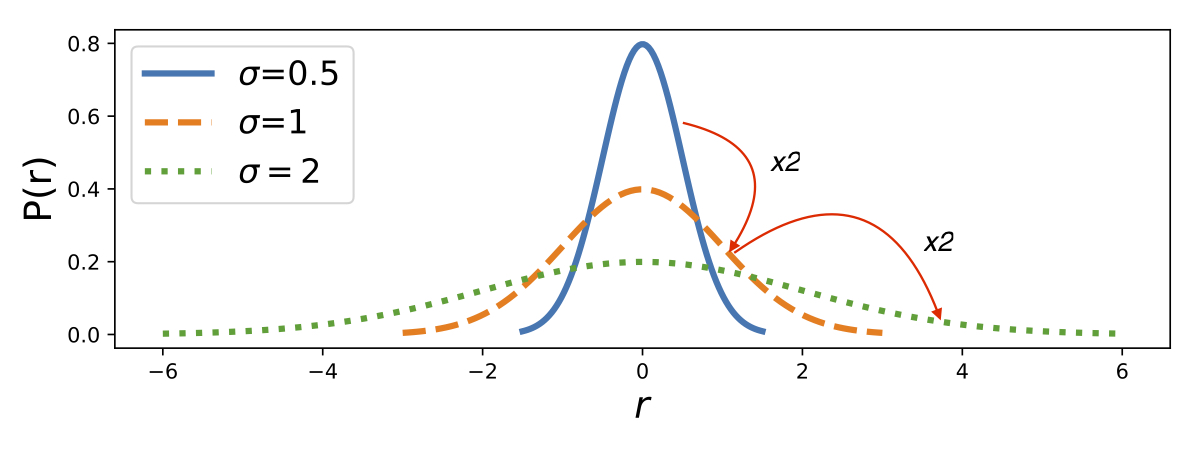
\includegraphics[width=0.8\linewidth]{ill/std_2.jpg}
  \vspace{-5pt}
  \caption{Illustration of the obfuscation effect brought by larger values of standard deviation $\sigma$.}
  \vspace{-5pt}
  \label{fig:std}
\end{figure} 

For the high utility of the obfuscated graph, smaller values of the parameter $r_{e}$ should be favored.  
The most widely known member of generating distribution $R({\sigma})$ is the truncated normal distribution with mean 0 and variance $\sigma^2$. 
In principle, $R$ could be any distribution.
As the standard deviation $\sigma$ decreases, a greater mass of $R_{\sigma}$ will concentrate near $r_{e}=0$.  
As illustrated in Figure~\ref{fig:std}, smaller values of $\sigma$ generally contributes towards better utility preserving, while at the same time they provide lower level of obfuscation. 
Larger values of $\sigma$ have the opposite effect.
Then, the amount of injected noise and consequent structural distortion will be smaller. 
Aiming at the high utility, {\soaName} aims at injecting the minimal amount of uncertainty need to achieve the necessary obfuscation. 
As outlined in Algo~\ref{alg:obf}, it computes the minimal amount of uncertainty via a binary search on the $\sigma$ value. 
\begin{algorithm}
    \begin{algorithmic}[1]
    	\item[] {\textbf{Input:}~Graph $\mathcal{G}$, obfuscation level $k$, tolerance parameter $\epsilon$}
        \item[] {\textbf{Output:}~The result $\mathcal{G}_{obf}$}
     	\STATE {$\sigma_{l} \leftarrow 0$; $\sigma_{u} \leftarrow 1$} \\
        \REPEAT
        \STATE{$\langle \hat{\epsilon}, \hat{\mathcal{G}} \rangle$ $\leftarrow$ \textbf{genObf}(-,$\sigma_{u}$)} \\
        \STATE{{\bf if} $\hat{\epsilon}=1$ (fail) {\bf then} $\sigma_{l} \leftarrow \sigma_{u}$; $\sigma_{u} \leftarrow 2\sigma_{u}$}
        \UNTIL{$\hat{\epsilon} \neq 1 $} \\
        \REPEAT
        	\STATE {$\sigma_{mid} \leftarrow (\sigma_{u}+\sigma_{l})/2$}
            \STATE{$\langle \hat{\epsilon}, \hat{\mathcal{G}} \rangle$ $\leftarrow$ \textbf{genObf}(-,$\sigma_{mid}$)}
            \STATE {{\bf if} $\hat{\epsilon} =1$~{\bf then}~$\sigma_{l} \leftarrow \sigma_{mid}$}\\
            \STATE {{\bf else} $\sigma_{u} \leftarrow \sigma_{mid}$;~~{$\mathcal{G}}_{obf} \leftarrow \hat{\mathcal{G}}$}
        \UNTIL{$\sigma_{u}-\sigma_{l}$ is enough small}
        % \COMMENT{\textcolor{blue}{\scriptsize Binary search for better obfuscation}}
        \STATE {return $\mathcal{G}_{obf}$}
    	\caption{The obfuscation algorithm}
	 \label{alg:obf}
    \end{algorithmic}
\end{algorithm}


The function {\genobf} determines the search flow. The function {\genobf} handles the search of {\keobf} instances using a given standard deviation parameter $\sigma$. It either returns the found sanitized instance or failure sign.
The search starts with an initial guess of an upper bound $\sigma_{u}$, which is iteratively doubled until a {\keobf} instance is found. Then, the binary search is performed over the range $[0,\sigma_{u}]$. The binary search terminates until the search interval is sufficiently short. The algorithm outputs the best found sanitized output  (the last one that was successfully generated; the one with the samllest $\sigma$).

\subsection{Genobf Function}
It is a difficult problem to find {\keobf} sanitized solutions using a given parameter $\sigma$ over the intractable search space. 
The function {\genobf} separate the search process into running two independent modules: (1) uncertain noise generative models and (2) privacy tests. 
The first constructs a utility-preserving noise generative model. 
By contrast, the privacy test aims to safeguard the privacy of generated obfuscation. 
It utilizes the random search to alleviate the combinational intractability.  
Multiple randomized attempts are performed. 
Every obfuscated output is subject to this privacy test. 
Iff all the attempts fail, {\genobf} returns failure sign. Otherwise, it returns the found {\keobf} instance.  

Each construction attempt begins with selecting a subset of edges subject to alteration. 
Then, it assigns the deviation among selected edges and injects uncertainty. 
While, the randomization process heavily relies on the heuristic.  
In particular, {\soaName} suggests calibrating the perturbation applied to an edge $e$ according to the ``uniqueness" of the two nodes $u$ and $v$. 
In brief, if both $u$ and $v$ are common nodes {\wrt} the property, then $r_{e}$ should be very small; 
on the other hand, if $u$ and $v$ are outliers, then $r_{e}$ should be higher. 
Meanwhile, edges need to be sampled with the higher probability if they are adjacent to outliers. 

\subsection{Limitations} 
The {\soaName} method achieves the desired level of obfuscation with the small change in the graph data, thus maintaining high utility.
However, this method has two critical weaknesses in the probabilistic context:
(1) The design heavily tailored towards the deterministic scenario {\eg} it assumes the existence of edges is binary (0,1). Thus, it fails to handle uncertain graphs where the existence of edges is probabilistic. 
All the operators, including edge selection and alteration, need to be integrated with possible world semantics carefully.
(2)  Its scheme does not consider the structural relevance of edges in critical edge selection/alteration steps, which leads to unnecessary structural distortion.
We are left asking the following questions, \emph{how to generalize existing methods to the probabilistic context?} and \emph{how to get a better trade-off between privacy and utility in the probabilistic context?} 